%\documentclass[linenum,doublespace,onecolumn]{SSA-SRL}
\documentclass[linenum]{SSA-SRL}
\pdfoutput=1
\switchlinenumbers* % SSA class + lineno v5 put numbers in the gutter; this restores outer margins

\usepackage{tikz}
\usetikzlibrary{positioning,arrows.meta,fit}

\citethisauthor{Thompson, G., J.~A. Power, R.~A. White, and W. McCausland}
\doi{00.0000/000000000}
\recdate{00 Month 0000}

\graphicspath{{./figures/}}

\newcommand{\file}[1]{\texttt{#1}}

\begin{document}

\title{Recovering the 1991 Mount Pinatubo Seismic and Monitoring Record: Clocks, a Linked Catalog, and Reproducible Workflows}

\author[*1\orc{0000-0002-9173-0097}]{Glenn Thompson}
\author[2]{John A. Power}
\author[3]{Randall A. White}
\author[4]{Wendy McCausland}

\affil[1]{School of Geosciences, University of South Florida, Tampa, Florida, U.S.A.}{\auorc[https://orcid.org/]{0000-0002-9173-0097}{(GT)}}
\affil[2]{Retired; formerly U.S. Geological Survey, Alaska Volcano Observatory, Anchorage, Alaska, U.S.A.}{}
\affil[3]{Retired; formerly U.S. Geological Survey, California Volcano Observatory, Menlo Park, California, U.S.A.}{}
\affil[4]{U.S. Geological Survey, Cascades Volcano Observatory, Volcano Disaster Assistance Program, Vancouver, Washington, U.S.A.}{}
\corau{*Corresponding author: thompsong@usf.edu}

\begin{abstract}
The seismic and monitoring data recorded during the 1991 eruption of Mount Pinatubo, Philippines, survived as triggered SUDS/DMX waveform files, analyst phase cards, two HYPO71 hypocenter summaries, and the BOB archive of RSAM, SSAM, tilt, rain, lahar, gas and count products. Each stream was time-stamped by its own acquisition computer, and those clocks used Philippine time or GMT at different times; the acquisition software also converted the seismic computer's clock as if it were in California. As recovered, the datasets disagreed by up to 15 hours, and only 12.9\% of hypocenters fell inside a waveform record. We reconstruct the clock history of every stream from file order, header fields and cross-correlation between products, encode it as a table of rules, and convert every time to Coordinated Universal Time (UTC) where it is read. After conversion 97.3\% of hypocenters fall inside a waveform record. A linked catalog of 21,753 events records which of waveforms (21,459 files, 152,933 traces), phase picks (58,068) and hypocenters (8,233 solutions in 4,690 groups) survive for each event, and is exported to QuakeML, SEISAN and CSS3.0. Regional and teleseismic arrivals in triggered records, matched to ISC and USGS origin times, show that residual clock errors reach $-$23 to $+$12~s after the main clock reset, so we assign a 25~s nominal uncertainty. On the common UTC time axis, triggered-event frequency content, catalog magnitudes, RSAM and SSAM from different computers can be compared directly; in early June 1991 the frequency index and spectral centroid of triggered events fall at two stations, and RSAM steps up at the time of the first large explosive eruption on 12 June. We describe the conversion and analysis workflows in full: open notebooks built on the FloVoPy library, with provenance, tests and a StationXML network history built once every stream is on UTC.
\end{abstract}

\maketitle

\section{Introduction}

Mount Pinatubo's 1991 unrest developed into one of the largest eruptions of the twentieth century while scientists of the Philippine Institute of Volcanology and Seismology (PHIVOLCS) and the U.S. Geological Survey (USGS) Volcano Disaster Assistance Program (VDAP) were still assembling the observations needed to assess the hazard. Monitoring and interpretation informed warnings and evacuations while the observatory itself faced changing access, telemetry failures and relocation \citep{Harlow_1996,Wolfe_1996}. The historical accounts in \textit{Fire and Mud} document the crisis, the network, the instruments and the acquisition software \citep{Newhall_1996}, but they do not replace the original observations. Reanalysis needs the waveform samples, analyst picks, location products, station histories and other monitoring measurements, and these were stored separately and survived unevenly.

The surviving holdings were assembled from copies retained by participants and released as EarthScope Assembled Dataset 25-028 (PIN 1991 FAIR), associated with temporary network XB (1991) \citep{XB_1991}. Recovering them involves more than translating an old file format. It requires documenting custody, separating original observations from derived products, and establishing which relationships between records the evidence supports. The Montserrat analog-network recovery is a precedent \citep{Thompson_2020}, but its timing control and metadata cannot be transferred to Pinatubo by analogy.

The largest obstacle turned out to be time. The Pinatubo Volcano Observatory (PVO) had no satellite or GPS time reference. Every data stream was stamped by the clock of the personal computer (PC) that acquired it, and those clocks were set to Philippine Standard Time (UTC$+$8) or to GMT at different times. The seismic acquisition software additionally converted its PC's wall-clock time as if the PC were in California. As recovered, waveforms, picks, hypocenters and amplitude summaries disagreed by up to 15~hr, and any catalog built from them silently failed to link most events.

This paper describes the recovered record and the work that turned it into a consistent archive. We summarize the monitoring system and the surviving products; reconstruct the clock history of every stream and convert every time to Coordinated Universal Time (UTC); bound the residual clock error with regional and teleseismic arrivals; describe in full the conversion workflow that produces the linked catalog, station metadata and monitoring products, and the analysis workflow that measures noise and event windows across the archive; and state what the archive can and cannot support. A physical reinterpretation of the precursory seismicity is left to separate studies.

\section{The 1991 Monitoring System}

\subsection{Network and telemetry}

PHIVOLCS's initial observations used portable recorders that were not part of the subsequent telemetered network. The VDAP deployment brought signals by radio to PVO at Clark Air Base. The field synopsis records a temporary Lily Hill installation on 25 April, PIE on 30 April, and CAB and UBO on 1 May; PPO, BUR, BUG and GRN followed during May, and PPO became a three-component station on 12 May \citep{Lockhart_1996}. By early June the recorded components were BUGZ, BURZ, CABZ, GRNZ, PIEZ, PPOZ, PPON, PPOE and UBOZ. The loss of the Bunker Hill link on 11 June interrupted several channels at once, and the climactic eruption on 15 June destroyed or isolated most sites. The later network recorded CAB, CRW, DON, FNG, PI2 and QAD in addition to BUG (Fig.~\ref{fig:network}). Dated radio-frequency maps from 14 May, 27 June and 8 July record discriminator slots, VCO subcarriers and relay paths, for example CRWZ relayed through PI2 and BUGZ through QAD.

\begin{figure*}
\centering
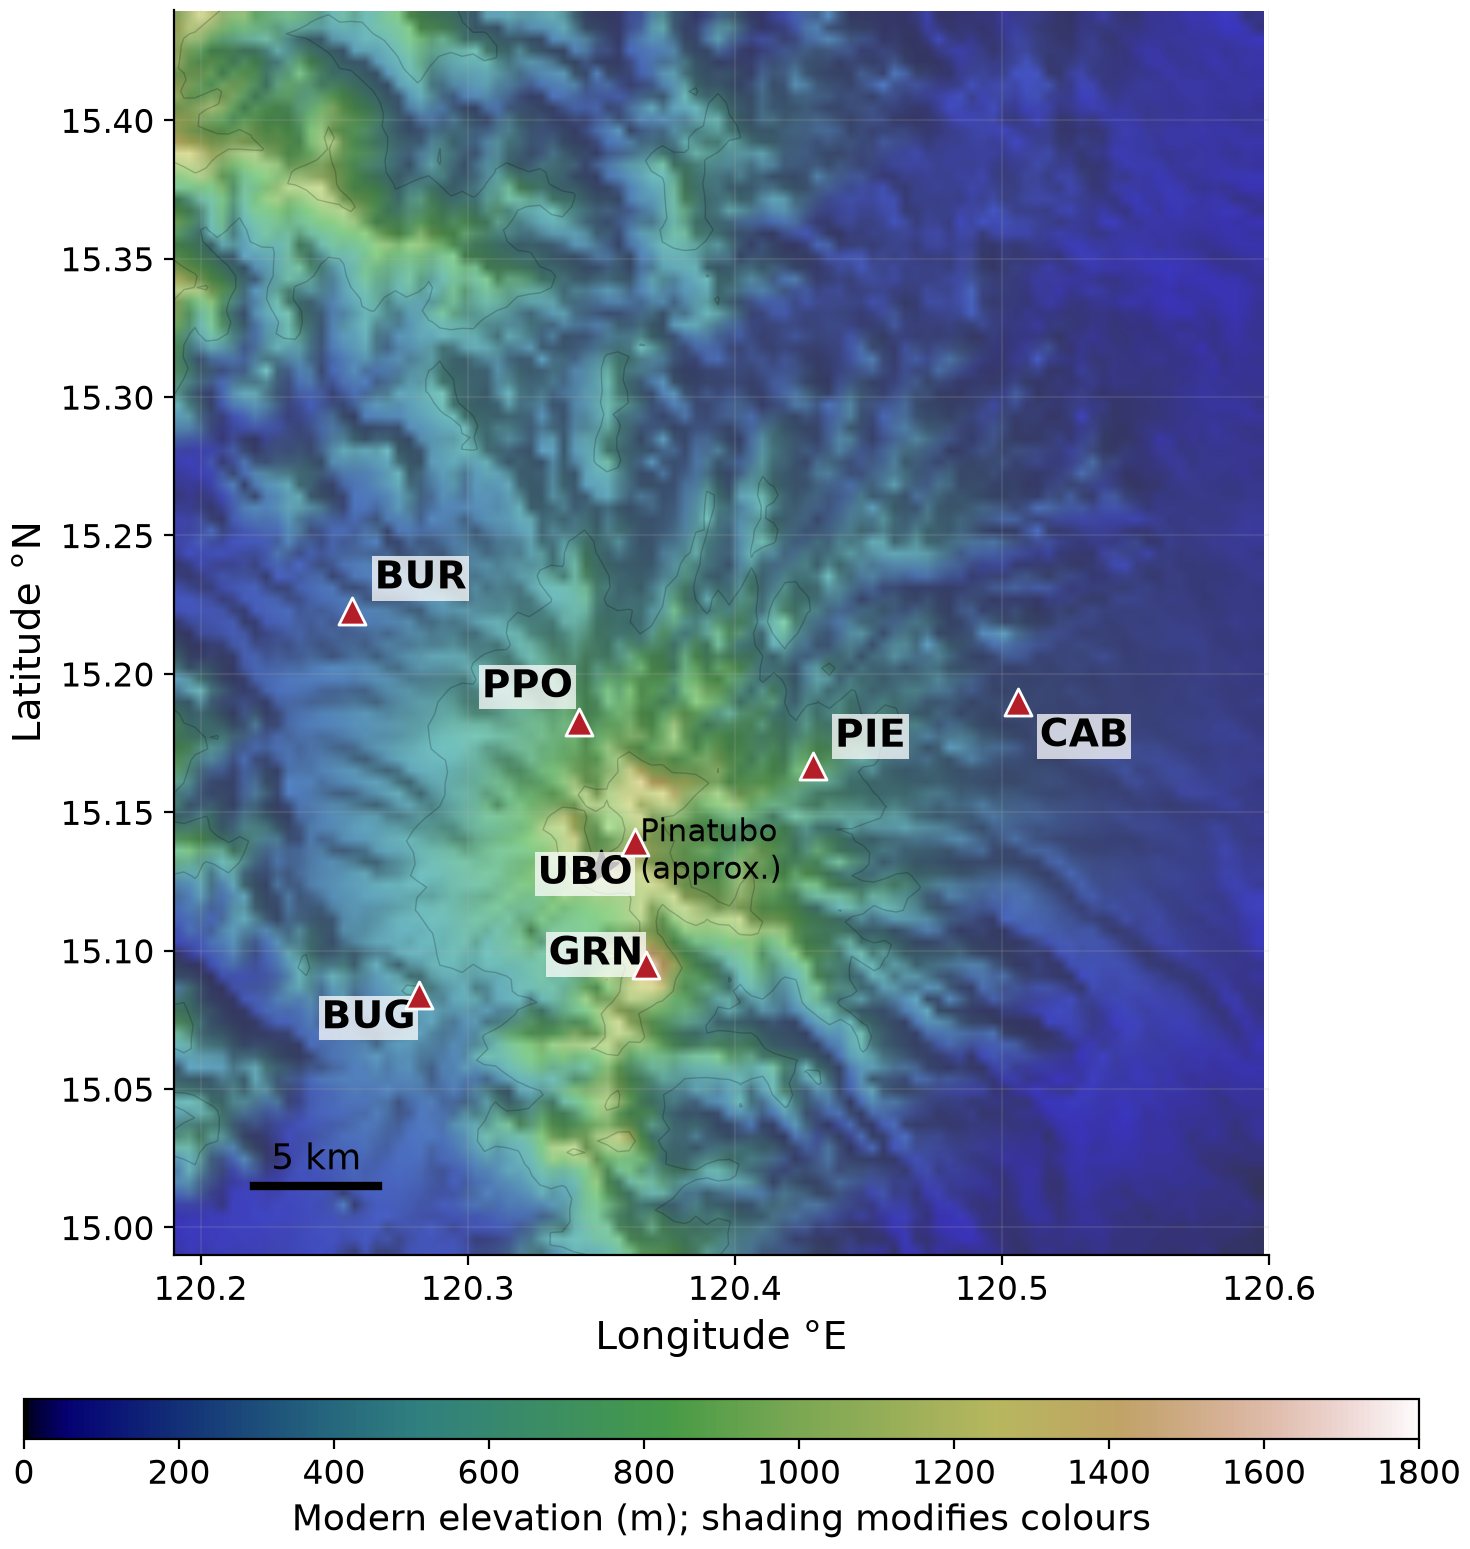
\includegraphics[width=0.48\textwidth]{fig_network_early}\hfill
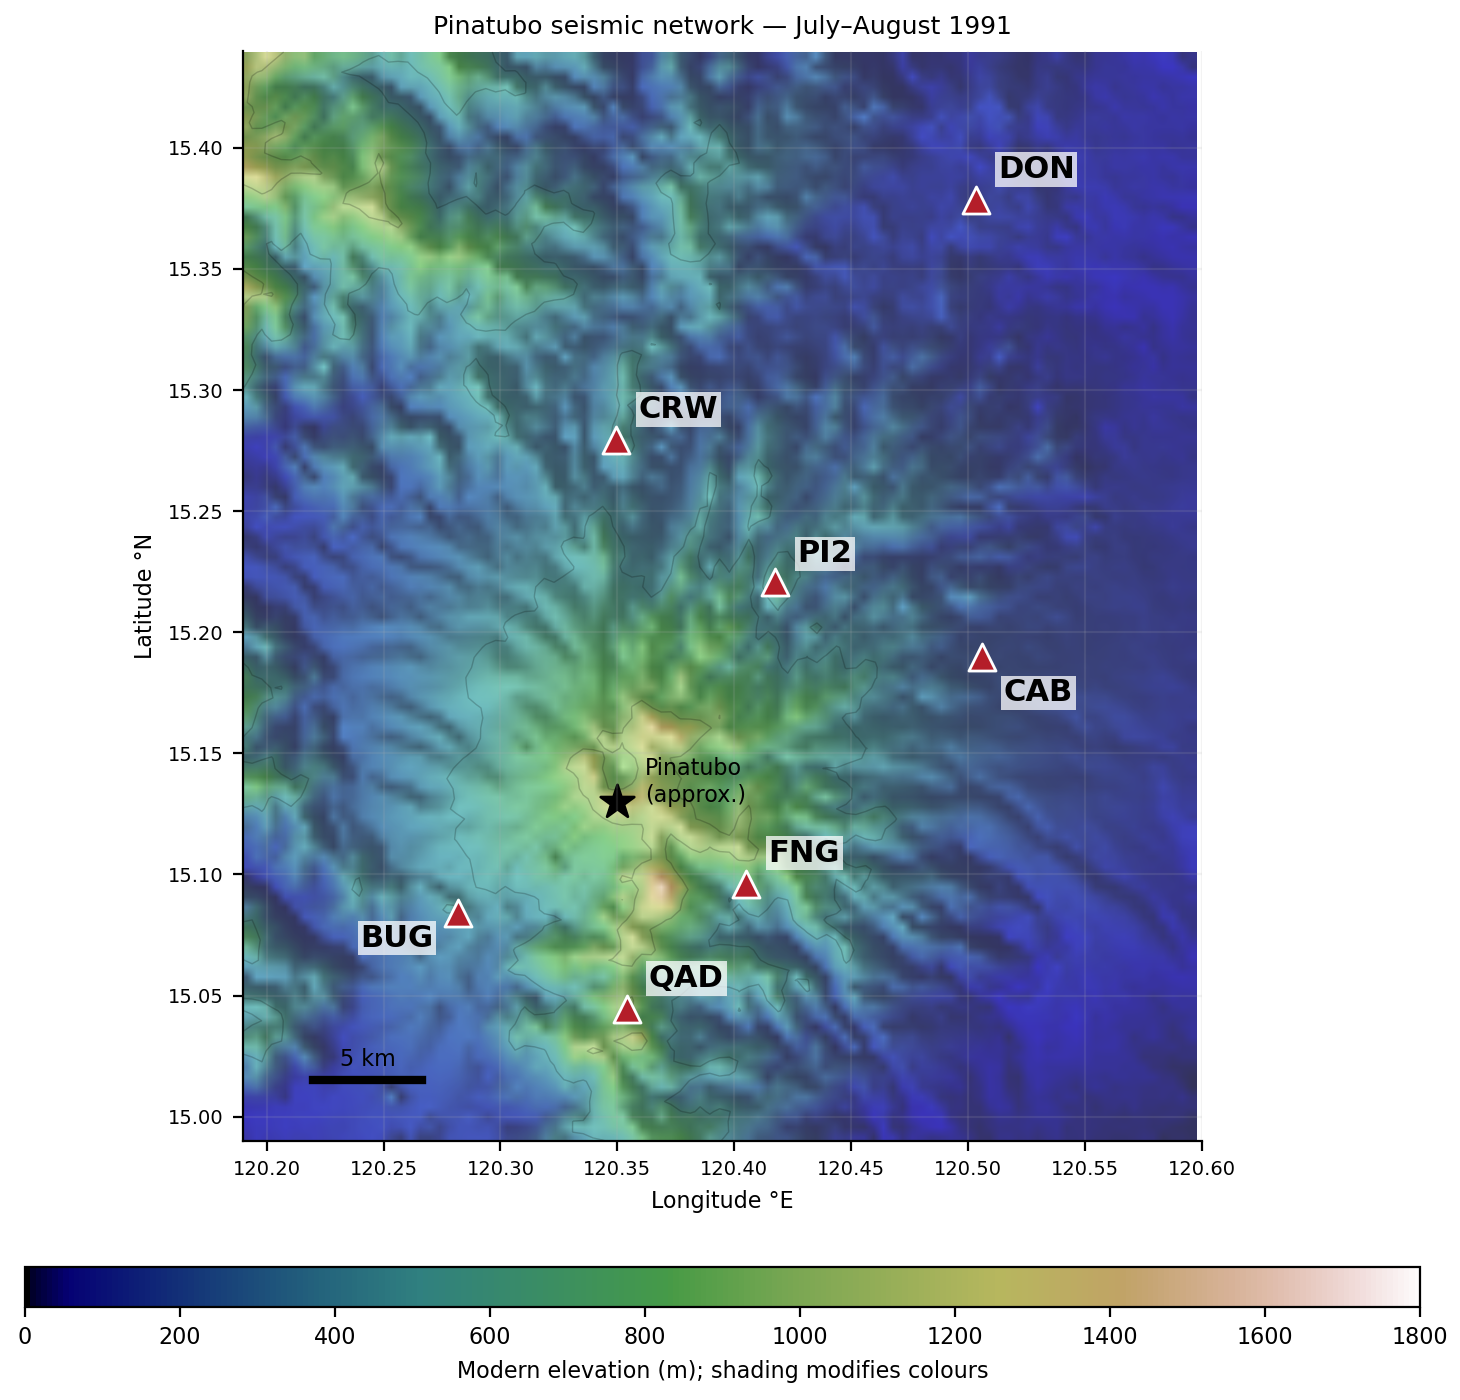
\includegraphics[width=0.48\textwidth]{fig_network_later}
\caption{Station configurations of the (a) initial network in early June and (b) later network in July--August 1991 (triangles; labels are legacy station names; star, approximate summit). Panel (b) shows every station identity found in July--August waveform headers; continuous operation and exact deployment dates are not verified. The background is modern 15-arcsec relief, not the 1991 surface. The datum of the historical coordinates is unresolved, and PVO and the repeater sites are not plotted because their positions are unverified. Outages and the 11 June losses are listed in the network history (step 70).}
\label{fig:network}
\end{figure*}

The early network combined vertical Mark Products L-4 sensors with a three-component L-22D at PPO. Field signals were frequency modulated, sent by radio, demodulated at PVO and passed to helicorders and to analog-to-digital converters on the acquisition PCs.

\subsection{Acquisition computers and their clocks}

The Mobile Monitoring System used several networked PCs \citep{Murray_1996}. Figure~\ref{fig:pvo} shows the data paths. Five PCs acquired data, and each stamped its products with its own clock:
\begin{itemize}
\item WILLIE (IBM-AT) ran MDETECT \citep{Lee_1988,Tottingham_1989}, which wrote triggered waveforms as PC-SUDS demultiplexed (DMX) files \citep{Ward_1989}, and SSAM, which averaged spectral amplitudes in 16 bands each minute \citep{Rogers_1995}.
\item A Tandy Model 100 ran RSAM \citep{Murray_1989}, which digitized discriminator outputs at 8 bits and reported 10-minute average amplitudes and EVNT counts of ``RSAM events'' (two-second amplitude jumps) on three channels.
\item SLEEPY (IBM-XT) logged tilt.
\item RICKY (IBM-XT) logged acoustic flow monitors for lahars, and, we infer, rainfall.
\item Analysts timed the waveforms with PCEQ \citep{Valdes_1989} and located earthquakes with HYPO71PC \citep{Lee_1985} on a second PC, SQUAB \citep{Murray_1996}, whose clock followed WILLIE's.
\end{itemize}
The aggregation PC (PORKY, or DAVE/ANDY) ran the BOB display and archive software \citep{Murray_1990}. It received the RSAM, tilt and lahar products through a buffered serial printsharer and SSAM from WILLIE, but its own clock stamped no data. A shared archive therefore does not imply a shared clock, and the clock of each product must be established separately.

\begin{figure*}
\centering
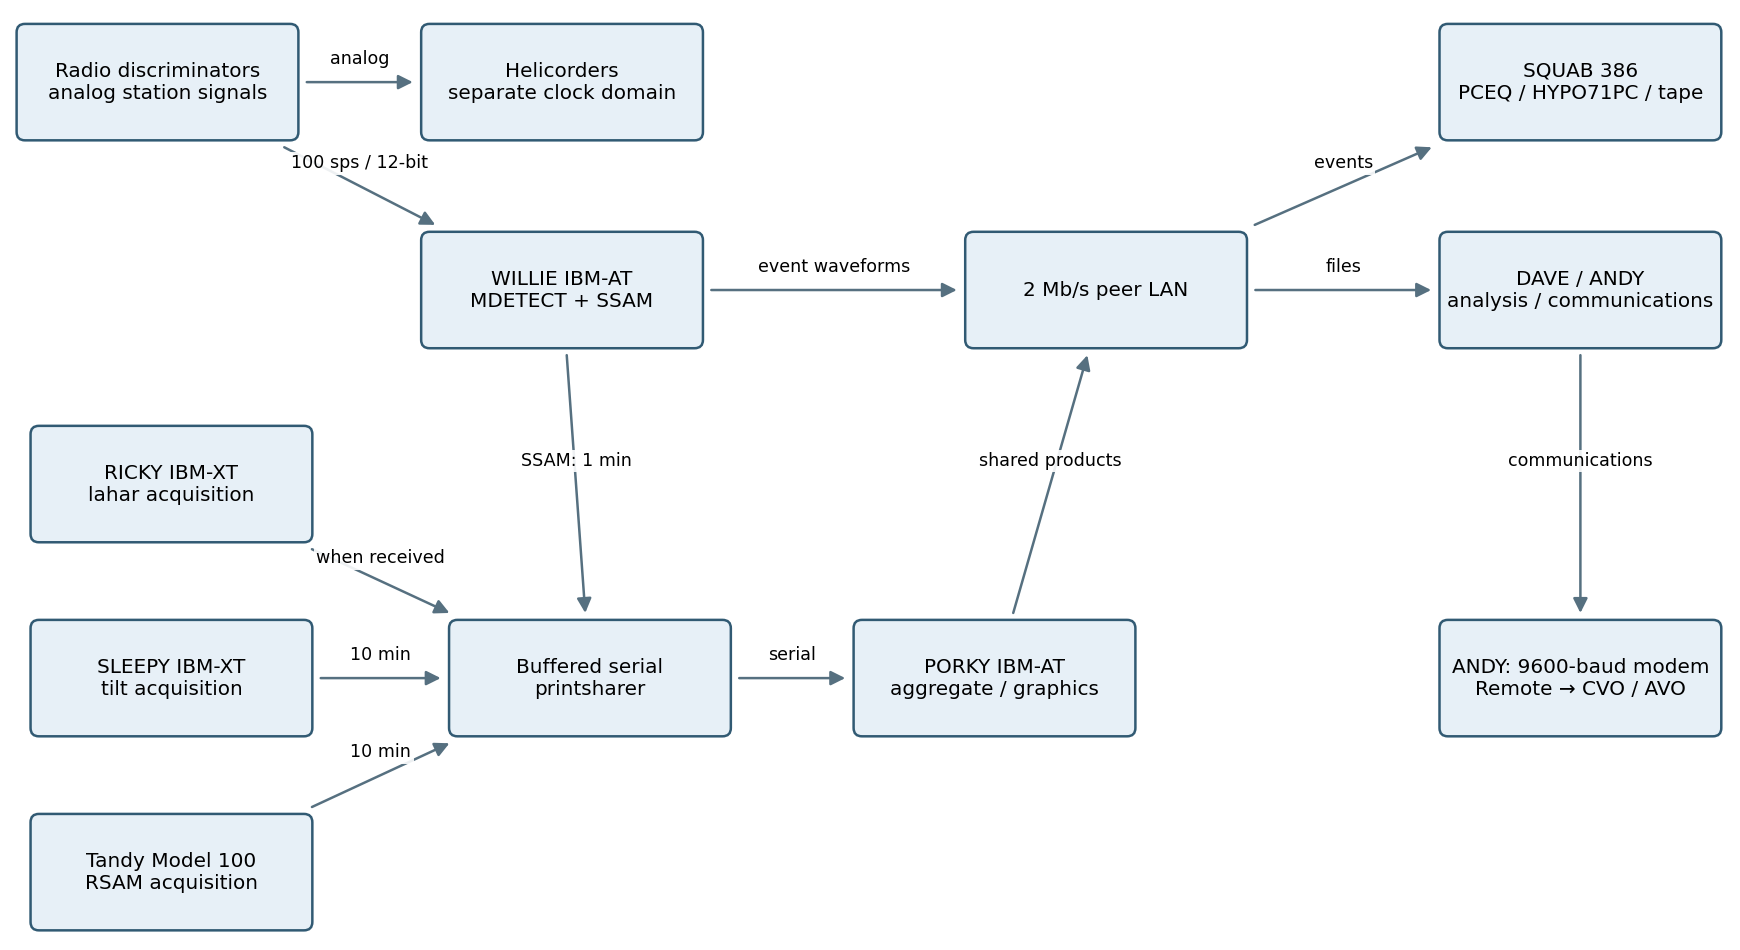
\includegraphics[width=0.9\textwidth]{fig_pvo_system}
\caption{The PVO data acquisition system in its initial 1991 configuration \citep[after][]{Murray_1996}; later software improvements are not assumed to be present from the start. Each acquisition PC (WILLIE, the Tandy RSAM computer, SLEEPY and RICKY) stamped its products with its own clock. The aggregation PC collected products but timed none of them, and neither aggregation nor LAN transfer synchronized the clocks. Labelled cadences describe products and transfers, not native sampling rates.}
\label{fig:pvo}
\end{figure*}

MDETECT read the PC clock at start-up and then kept time by counting samples, ``good to about 2 seconds per day'' \citep{Lee_1988}. The PC clocks were set by hand to WWV radio time signals and the PCs were meant to be rebooted daily, but this was often not done in the first weeks, and the PC and RSAM clocks were found on several occasions to have drifted by several minutes \citep{Lockhart_1996}. A GOES satellite clock was on hand but could not receive signals in the Philippines, no GPS clock was in use, and the IRIG time code recorded on one channel came from a free-running generator, so it gives no absolute time.

\section{Surviving Products}

Table~\ref{tab:inventory} lists the surviving products and the standardized derivatives produced here. Digital acquisition saved triggered windows rather than continuous data: each DMX file represents a detector decision and a finite window, typically 50--80~s, that starts about 11~s before the triggering arrival. File absence therefore does not establish seismic quiet, and a window can contain several earthquakes. The analyst record survives as 119 single-event phase files (3--16 June), four monthly phase files (May--August), and two HYPO71 summaries: \file{Pinatubo\_all.sum} (4,632 origins) and \file{PINAALL.DAT} (3,601 origins). Neither summary is authoritative; they share many events with slightly different solutions. A recovered set of HYPO71 control cards from June 1991 gives the station coordinates and a five-layer velocity model with $V_P/V_S = 1.78$.

\begin{table*}
\tbl{Surviving products, their legacy form, the standardized derivative, and the principal remaining qualification.\label{tab:inventory}}
{\begin{tabular*}{\textwidth}{@{\extracolsep{\fill}}p{0.17\textwidth}p{0.2\textwidth}p{0.29\textwidth}p{0.26\textwidth}@{}}
\toprule
\textbf{Product} & \textbf{Legacy form} & \textbf{Standardized derivative} & \textbf{Main qualification} \trowsep
Triggered waveforms & 21,475 PC-SUDS DMX files & MiniSEED in a SEISAN WAV database; waveform index; per-file log & Trigger selection; clipping; nominal response only \trowsep
Phase picks & Single-event and monthly PHA files & Merged pick index; picks in QuakeML, SEISAN REA and CSS3.0 & Duplicates across sources; S readings after the minute \trowsep
Hypocenters & \file{Pinatubo\_all.sum}, \file{PINAALL.DAT} & Origin and event indexes; preferred origins; QuakeML & Not relocated; quality and depth datum as reported \trowsep
Station metadata & Field notes, maps, HYPO71 cards & Network history; StationXML on UTC & Nominal sensor model; electronics unknown \trowsep
RSAM, EVNT & BOB annual binary files & 10-min tables with window start and end & Legacy amplitude units; EVNT counts channel triggers \trowsep
SSAM & Daily 16-band text files & 1-min tables, dropouts flagged & Band scaling; one-minute labels \trowsep
Tilt, rain, mudflow & BOB annual binary and daily text & Tables with saturation, carried-value and gap flags & Calibration; rain and mudflow after 15 Nov unverified \trowsep
COSPEC, counts, radio maps & Hand-entered text & Dated tables & Dates only, no time of day \trowsep
Helicorders & 143 scanned drum records & Image inventory \citep{Power_2025} & No digitized waveforms; separate clock \\
\botrule
\end{tabular*}}
{}
\end{table*}

The BOB archive holds products beyond seismology. Their coverage, after conversion to UTC, is shown in Figure~\ref{fig:bob}: RSAM and EVNT on 206 days (19 April--22 November), SSAM on 135 days (1 June 1991--21 March 1992), counts on 178 days, rain on 122 days, mudflow on 121 days, COSPEC on 17 days and tilt on 14 days (31 May--13 June). A represented day requires one recovered, non-missing value on one channel; it does not mean continuous operation. Scanned helicorder drum records (143 images of PIE, UBO and CAB, 30 April--17 June) are preserved separately \citep{Power_2025}; they carry Philippine local time from an independent recorder clock and are not used in the digital catalog.

\begin{figure*}
\centering
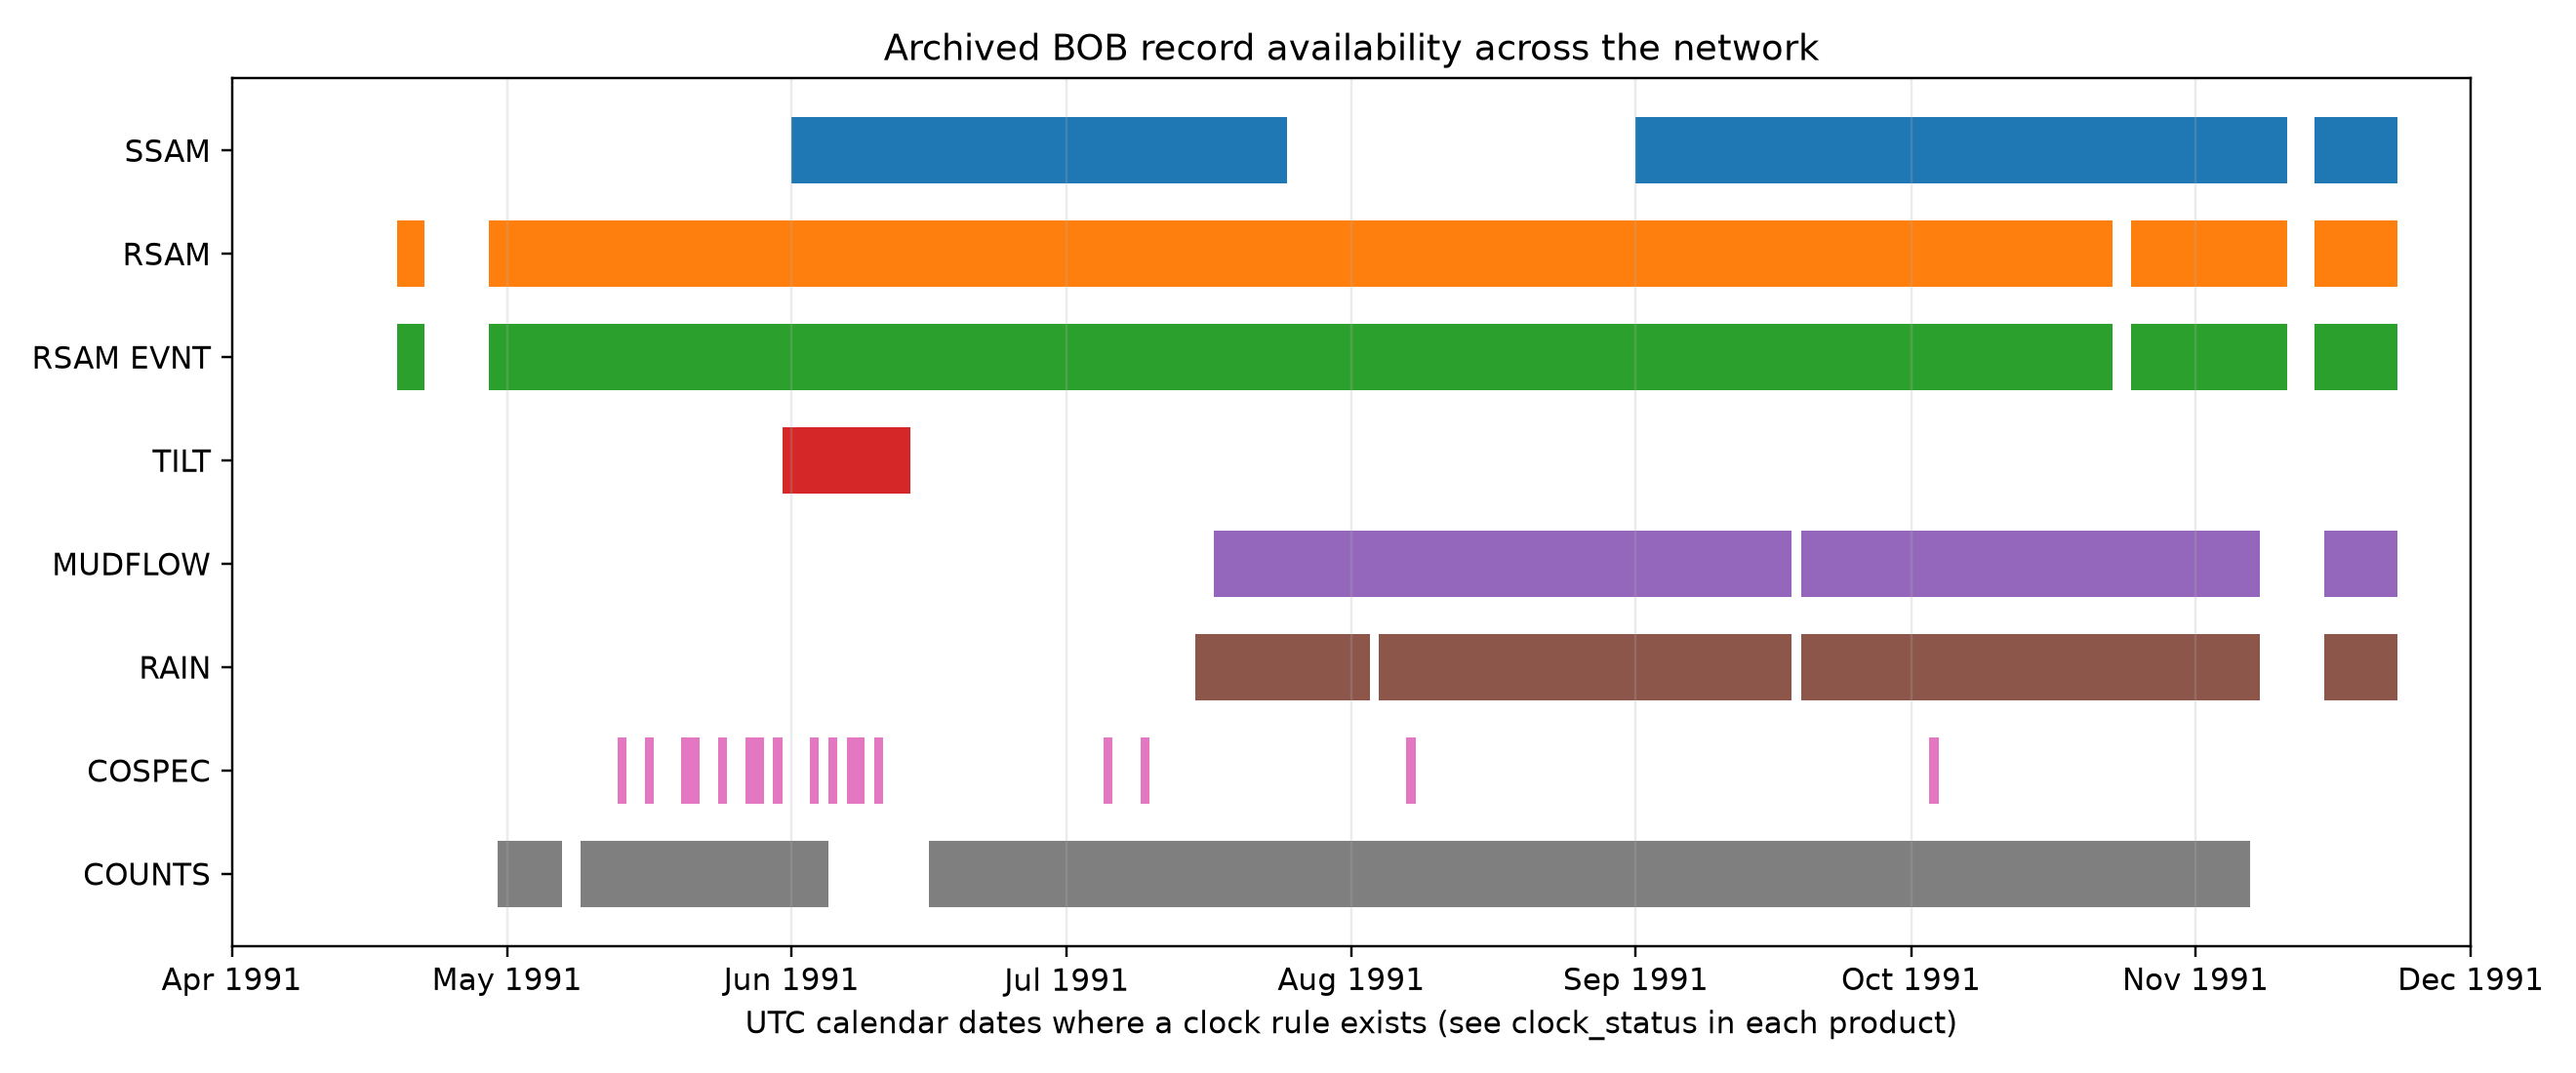
\includegraphics[width=0.9\textwidth]{fig_bob_coverage}
\caption{Network-wide coverage of the BOB products on UTC days. Each row is the union across channels; gaps remain visible. A represented day needs one non-missing value on one channel. COSPEC, the daily PIE counts and the radio maps carry dates only.}
\label{fig:bob}
\end{figure*}

\section{Reconstructing the Clocks}

\subsection{The problem}

Before any correction, the four main streams disagreed. Waveform start times and hypocenter origins were offset by about 7~hr, so that only 12.9\% of origins fell inside a waveform record (Fig.~\ref{fig:timing}). Picks from the monthly phase files agreed with the waveforms in May and early June but not later. RSAM labels matched the waveforms neither in May nor in June. Because these offsets are hours rather than seconds, they are systematic, and they can be traced to how each system kept time.

\subsection{Three clocks on the seismic PC}

We distinguish the DMX header time H, as read by ObsPy \citep{Beyreuther_2010,Krischer_2015}, from W, the wall clock of WILLIE. Five independent lines of evidence show that MDETECT converted W to an epoch as if the PC were in California, using the DOS default time zone \texttt{TZ=PST8PDT}: H $=$ W $+$ 7~hr during U.S. Pacific daylight time and W $+$ 8~hr after daylight time ended at 02:00~PDT on 27 October 1991.
\begin{itemize}
\item From 26 May, each DMX filename date equals the date of H $-$ 7~hr, and of H $-$ 8~hr from 28 October.
\item Hypocenter origins, which analysts computed on W, equal H $-$ 7~hr in every week from May to August: 82--100\% of origins have a waveform record starting 0--20~s before origin $+$ 7~hr, while offsets of 0, 6, 8 and 9~hr give chance-level matches.
\item The lag of maximum cross-correlation between EVNT counts and the waveform trigger rate steps from $-$7 to $-$8~hr on the same date as the filename change.
\item J. Power (written comm., 2026) recalls that MDETECT ``always assumed that the computer was in California and corrected the time to GMT.''
\item \citet{Murray_1996} report that MDETECT stamped event data with the PC clock plus 8~hr, ``the time correction needed for G.m.t. in California,'' but SSAM data with the PC clock alone, and that several weeks passed before the discrepancy was resolved and all seismic data were recorded in GMT.
\end{itemize}

WILLIE's wall clock itself was on Philippine time until 26 May and on GMT afterwards. In the original file order, file \file{91052617} (H 15:41) is followed by \file{9105261G} (H 08:40): the clock went back 8~hr. \file{PINAALL.DAT} jumps back at the same point, from line 217 (08:31) to line 218 (01:40), and line 218 plus 7~hr is file \file{9105261G}. The SUDS trace descriptor field \texttt{localtime} is 0 in every file up to \file{91052617} and $-$25,200~s ($-$7~hr) from \file{9105261G} onward, through December: a new MDETECT version was installed at the reset, consistent with Power's recollection that H. Harlow installed one and set the clock to GMT ``on or about May 25'' \citep[see also][]{Murray_1996}. The data place the reset at about 00:41--01:40 UTC on 26 May, so wall-clock times between about 00:41 and 08:41 on that day occur twice. Waveforms in that window are resolved by requiring the header marker and the file order to agree, which they do for all 21,459 files; picks and \file{PINAALL.DAT} records are resolved by line order; and the 18 records of the time-sorted \file{Pinatubo\_all.sum} in the window are matched to \file{PINAALL.DAT} (13 records) or to the waveform file that covers them (5).

The phase picks switched clocks in June. The single-event phase files (3--16 June) and the monthly picks up to 10 June are on H: all fall inside waveform records at zero offset. From 27 June the monthly picks are on W, and 88--100\% fall inside waveform records once 7~hr is added. The switch lies in a gap with no picks between 10 and 27 June that contains a new set of HYPO71 control cards.

\subsection{The other acquisition computers}

The BOB products were each tested against a stream already verified in UTC.
\begin{itemize}
\item \textbf{RSAM and EVNT} (Tandy). Cross-correlating EVNT counts with the waveform trigger rate shows that the labels were Philippine time from 9 May to about 09:00 on 13 September ($\pm$3~hr) and GMT afterwards, consistent with the eruption onsets of 12 and 15 June. Each 10-minute value is labeled at the end of its window: EVNT counts match the waveform triggers in the preceding 10 minutes. On 10 November one block of labels (01:20--22:20) is on Philippine time again. From 2 to 9 May the labels equal H, which we cannot explain; that rule has low confidence.
\item \textbf{SSAM} (WILLIE). Station by station, SSAM labels are 8~hr behind RSAM until 13 September and match it afterwards (correlation coefficient $r = 0.72$--0.99), so SSAM was on GMT from its first data on 1 June, like WILLIE after the reset; MDETECT stamped SSAM with the PC clock \citep{Murray_1996}.
\item \textbf{Mudflow and rain} (RICKY). Despite file headers saying ``converted from GMT to local,'' mudflow amplitudes match RSAM at $-$8~hr until 12 September ($r = 0.4$--0.7) and at 0~hr from 15 September; rain matches mudflow at 0~hr throughout. Files from 15 November have a new format and nothing to test against, so their labels are kept and flagged unverified.
\item \textbf{Hourly CAB counts}, entered by hand, match EVNT at $-$8~hr until 13 September and at 0~hr afterwards, despite a ``TIME IN GMT'' header.
\item \textbf{Tilt} (SLEEPY) was rewritten to local time in November 1991 (a note records a phase shift of 48 ten-minute samples), and battery-voltage charging starts at the 07:00 label and peaks at 11:00--14:00 each day, so the labels are Philippine time.
\item \textbf{COSPEC, daily PIE counts and radio maps} carry dates only. COSPEC dates are taken as Philippine days, because the measurements were made in daylight; the PIE counts correlate equally well with EVNT on Philippine or UTC days.
\end{itemize}
RSAM, mudflow and CAB counts all switch from Philippine time to GMT around 13 September. These were separate computers, so the switch looks like an operational decision rather than one shared clock.

\subsection{Rules and their application}

The reconstructed history is encoded in a table (\file{clock\_regimes.csv}) with one row per stream and period: the raw-clock interval, an optional sequence bound and header marker, the offset to UTC, a nominal absolute uncertainty, a confidence label and the evidence. Figure~\ref{fig:clockrules} shows the rules, and Table~\ref{tab:corrections} summarizes them. A generic engine in FloVoPy (\file{flovopy.core.clock}) applies the table, rejecting records that match no rule or more than one; each conversion step applies it where it reads the raw times. Every product keeps the raw time in a \texttt{raw\_*} column next to the corrected one, with the applied rule and its nominal uncertainty; QuakeML origins carry the uncertainty as \texttt{time\_errors}.

\begin{figure*}
\centering
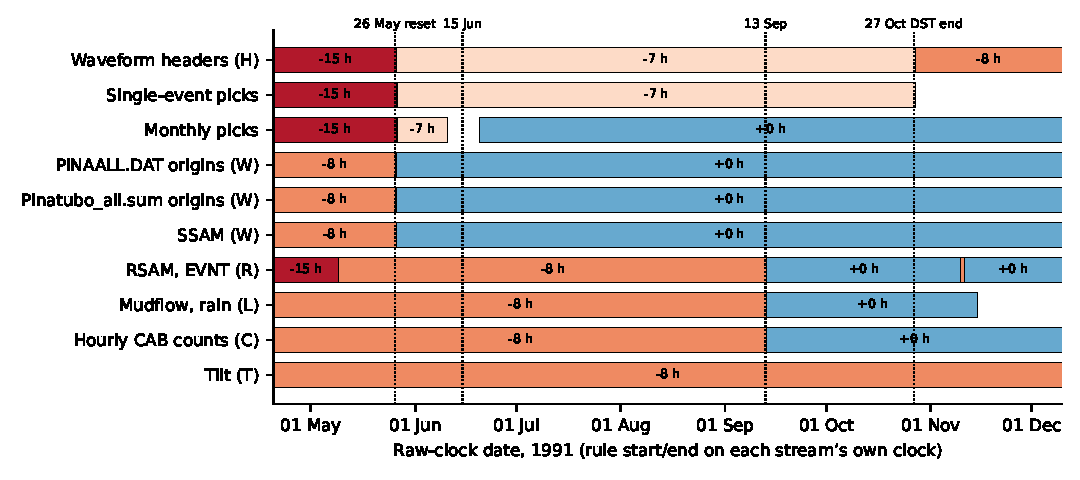
\includegraphics[width=\textwidth]{fig_clock_rules}
\caption{Clock rules by data stream: the offset added to each raw time to obtain UTC. Rule boundaries are on each stream's own raw clock. H, W, R, L, C and T are the clocks of the DMX headers, WILLIE's wall clock, the Tandy RSAM computer, RICKY, the hand-entered CAB counts and SLEEPY. Short rules resolving the repeated hours of 26 May by file or line order are omitted.}
\label{fig:clockrules}
\end{figure*}

\begin{table*}
\tbl{Corrections applied (raw time $+$ correction $=$ UTC) and nominal absolute uncertainties.\label{tab:corrections}}
{\small\begin{tabular*}{\textwidth}{@{\extracolsep{\fill}}p{0.25\textwidth}lp{0.15\textwidth}p{0.17\textwidth}p{0.15\textwidth}p{0.1\textwidth}@{}}
\toprule
\textbf{Data} & \textbf{Clock} & \textbf{Before 26 May} & \textbf{26 May--27 Oct} & \textbf{After 27 Oct} & \textbf{Uncertainty} \trowsep
Waveforms (DMX headers) & H & $-$15 hr & $-$7 hr & $-$8 hr & 60 s; 25 s after reset \trowsep
Single-event picks; monthly picks to 10 Jun & H & $-$15 hr & $-$7 hr & -- & as waveforms \trowsep
Monthly picks from 27 Jun & W & -- & 0 & 0 & 25 s \trowsep
Hypocenters (both summaries) & W & $-$8 hr & 0 & 0 & 60 s; 25 s after reset \trowsep
SSAM & W & (no data) & 0 & 0 & 60 s \trowsep
RSAM, EVNT & R & $-$15 hr (2--9 May); $-$8 hr & $-$8 hr to 13 Sep, then 0 & 0 ($-$8 hr on 10 Nov) & 300 s \trowsep
Hourly CAB counts & C & (no data) & $-$8 hr to 13 Sep, then 0 & 0 & 1800 s \trowsep
Rain, mudflow & L & (no data) & $-$8 hr to 13 Sep, then 0 & 0 to 15 Nov; unverified after & 600 s \trowsep
Tilt & T & (no data) & $-$8 hr & (no data) & 3600 s \\
\botrule
\end{tabular*}}
{}
\end{table*}

The effect is large (Fig.~\ref{fig:timing}). The fraction of hypocenter origins inside a waveform record (from 10~s before its start to its end) rises from 12.9\% on the recorded clocks to 97.3\% on UTC, and is above 89\% in every week. By month, picks inside waveform records rise from 77\% to 99.4\% in June and from 10--14\% to 95--98\% in July and August. EVNT matches the waveform trigger rate at zero lag in every window from May to December.

\begin{figure*}
\centering
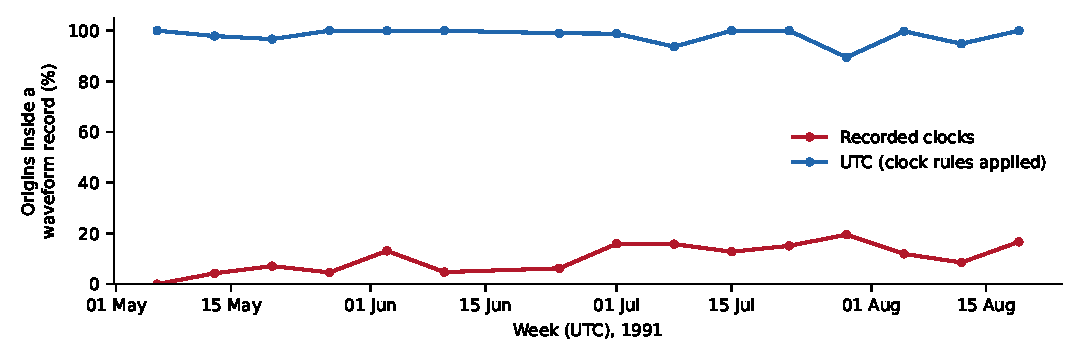
\includegraphics[width=\textwidth]{fig_timing_effect}
\caption{Weekly fraction of the 8,233 hypocenter origins that fall inside a waveform record (from 10~s before its start to its end), using the recorded clocks of both products (red) and after converting both to UTC (blue).}
\label{fig:timing}
\end{figure*}

\subsection{Drift between computers}

The rules remove hour-scale offsets, not drift. Comparing RSAM with summed SSAM bands day by day measures the Tandy clock against WILLIE's directly (Fig.~\ref{fig:drift}). Of 465 station-days from 1 June to 22 November, 412 correlate with $r \ge 0.5$, and 411 of those lie within 4 minutes of zero lag after the rules are applied. The lag moves in a sawtooth, growing by about a minute a day and then jumping back when one of the computers was restarted. This drift is not corrected; it is within the 300~s uncertainty assigned to RSAM labels.

\begin{figure*}
\centering
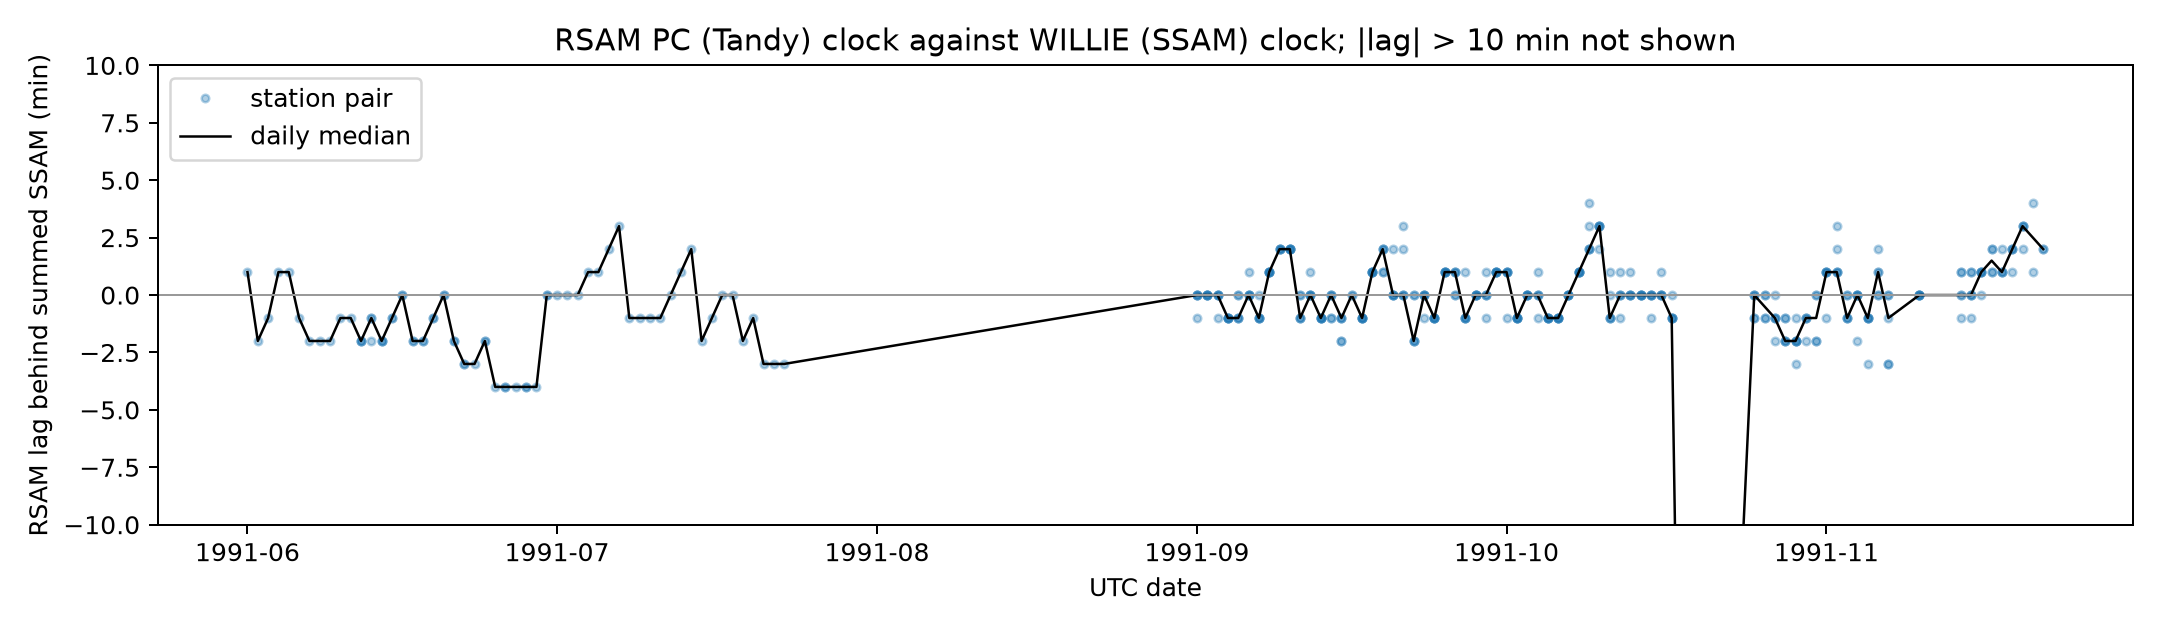
\includegraphics[width=\textwidth]{fig_ssam_rsam_lag}
\caption{Daily lag between RSAM (Tandy clock) and the 10-minute mean of summed SSAM bands (WILLIE clock), per station pair (dots) and daily median (line), on UTC. The sawtooth is drift between the two computers, reset when one was restarted. Lags beyond $\pm$10~min are not shown.}
\label{fig:drift}
\end{figure*}

\subsection{Absolute clock anchors}

Within one waveform file, relative timing is good to a sample, and because the picks and hypocenters were made from the same PC's waveforms, drift does not affect how they associate. It does affect their absolute time. Without an external reference, the only independent absolute times are arrivals of earthquakes whose origin times are known from global networks. We searched for them systematically (conversion step 72):
\begin{enumerate}
\item We downloaded ISC \citep{ISC_2024} and USGS \citep{USGS_2017} events for May--November 1991 within 6$^\circ$ of Pinatubo ($M \ge 3$) and worldwide ($M \ge 6$), merged duplicates, and predicted first-P arrival times at Pinatubo with TauP \citep{Crotwell_1999} in iasp91 \citep{Kennett_1991}.
\item None of the 8,233 HYPO71 origins lies beyond 49~km of the volcano, and the largest magnitude is 1.88, so the local catalog holds no regional events. Of the 84 global-catalog events within 80~km, mostly Pinatubo's own $M$~4--6 earthquakes, most fall on 15--17 June, when HYPO71 has no solutions; after the reset, the nearest HYPO71 origins differ from the global origins by tens of seconds (closest $-$10, $-$17 and $+$22~s). With global depths fixed at 10--35~km and one or two local events per minute, this rules out minute-scale errors but cannot measure seconds.
\item Thirty-four pick groups have median S$-$P times of 6--13~s (about 50--105~km), but none is in the global catalogs.
\item One-minute SSAM shows no network-wide rise at the predicted arrival of any of 45 distant events, including $M$~7.2 at 5,000~km.
\item The predicted P of 39 distant events falls within $\pm$120~s of a triggered record. We plotted every record holding a predicted P from an event of $M \ge 4.5$ with all predicted phases marked, and an analyst reviewed them (Fig.~\ref{fig:anchors}).
\end{enumerate}

Six records show a distant arrival with low frequency and little moveout across the network (Table~\ref{tab:anchors}). Two independent events on 30 May, a regional $M$~4.6 at 591~km depth 100~km and an $M$~7.0 off the Alaska Peninsula, both arrive about 12~s after their predicted P. The Alaska event alone could be a weak P followed by pP ($+$10~s) or sP ($+$15~s), but the regional event has no phase that early. Later anchors give $-$23~s (8 August), $+$4~s relative to pP (15 August; the predicted P precedes the record) and $+$9~s (5 September). Before the reset, a teleseism on 21 May arrives 40~s before its predicted P. The offsets change sign from day to day, as expected for drift of about 2~s per day with occasional restarts, so no correction is applied. Four of the five post-reset anchors exceed the 5~s uncertainty that MDETECT's specification would suggest, so we assign 25~s after the reset and keep 60~s before it.

\begin{table}
\tbl{Clock anchors from distant earthquakes in triggered records. Offset is the first clear arrival minus the predicted arrival of the reference phase; positive means waveform times are late (the clock was fast).\label{tab:anchors}}
{\begin{tabular*}{\columnwidth}{@{\extracolsep{\fill}}llll@{}}
\toprule
\textbf{Date (1991)} & \textbf{Record} & \textbf{Event} & \textbf{Offset} \trowsep
21 May$^{a}$ & 9105220C & $M$ 6.6, 2,602 km & $-$40 s \trowsep
30 May & 9105300K & $M$ 4.6, 591 km & $+$12 s \trowsep
30 May & 9105301M & $M$ 7.0, 7,863 km & $+$12.5 s \trowsep
8 Aug & 91080826 & $M$ 5.0, 351 km & $-$23 s \trowsep
15 Aug & 91081528 & $M$ 6.3, 6,272 km & $+$4 s (pP) \trowsep
5 Sep & 9109055G & $M$ 4.9, 420 km & $+$9 s \\
\botrule
\end{tabular*}}
{$^{a}$Before the 26 May reset.}
\end{table}

\begin{figure*}
\centering
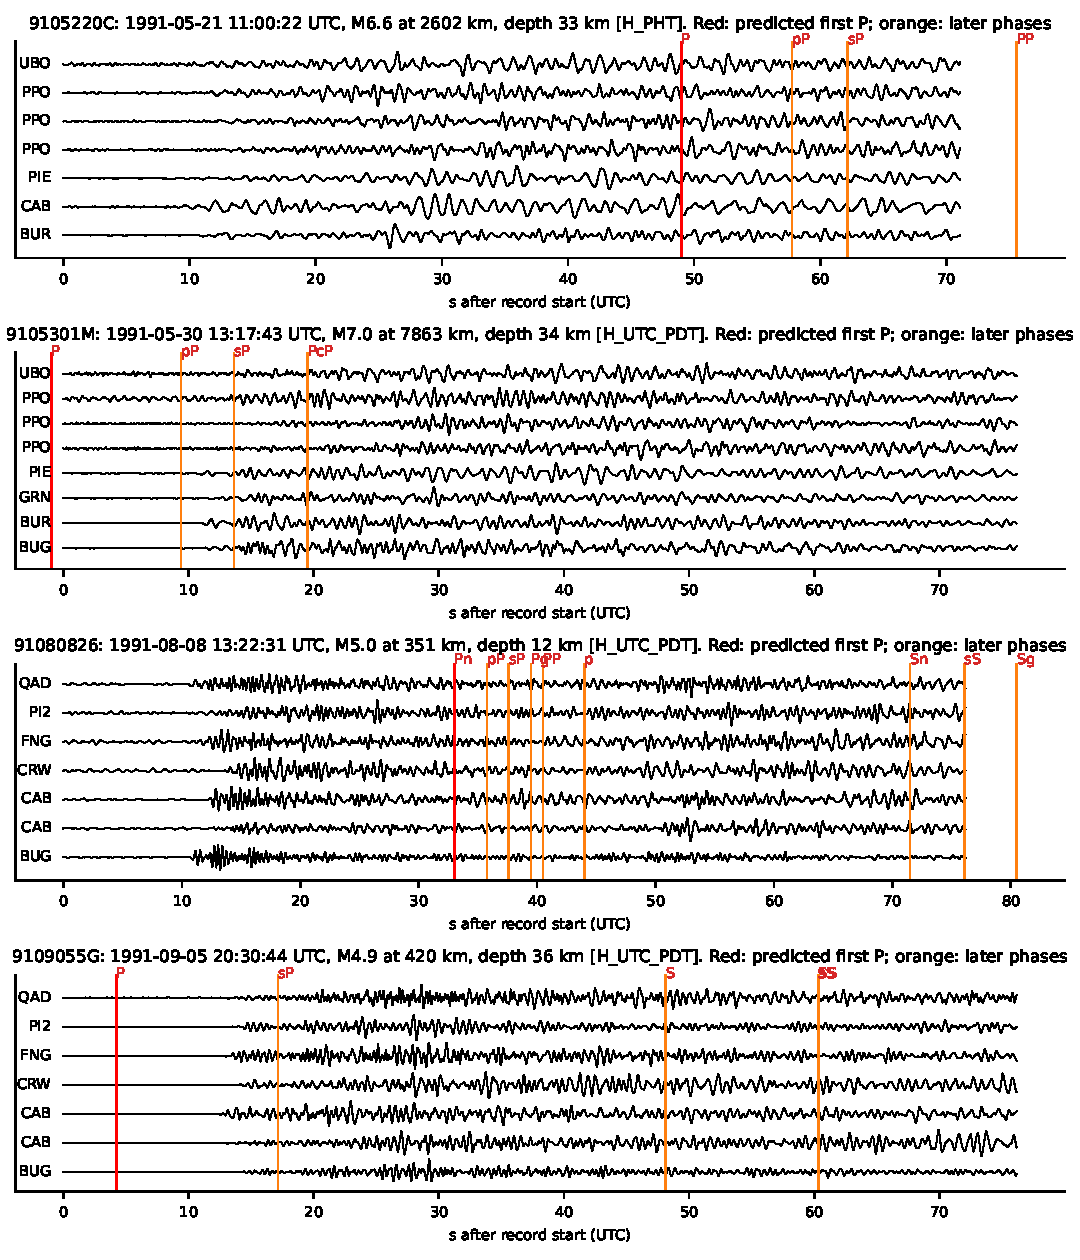
\includegraphics[width=0.95\textwidth]{fig_clock_anchors}
\caption{Four of the reviewed records, filtered 0.5--3~Hz, vertical components, with the predicted first P (red) and later phases (orange) of the matched ISC/USGS event. (a) 21 May, before the reset: the teleseismic wavetrain precedes the predicted P by about 40~s. (b) 30 May: first clear arrival about 12~s after the predicted P. (c) 8 August: onset about 23~s before the predicted Pn. (d) 5 September: onset about 9~s after the predicted P.}
\label{fig:anchors}
\end{figure*}

\section{Conversion Workflow}

The conversion is a sequence of numbered Jupyter notebooks in the \file{10\_conversion} folder of the project repository (Table~\ref{tab:steps}, Fig.~\ref{fig:workflow}). Each notebook has a configuration cell, a definitions cell holding only functions (tagged so tests can load it without running the notebook) and run cells. Paths come from one configuration file; outputs go outside the repository. Code that would serve any VDAP-era archive lives in the open-source FloVoPy library: DMX reading and conversion, partial-file recovery, phase-card decoding and pick clean-up, HYPO71 parsing, the clock-rule engine, SEISAN REA export, BOB readers and spectral methods. Pinatubo decisions (paths, clock rules, station mappings, association and export policies) stay in the notebooks and a small local package. The committed notebooks keep their outputs from the UTC run.

\begin{figure*}
\centering
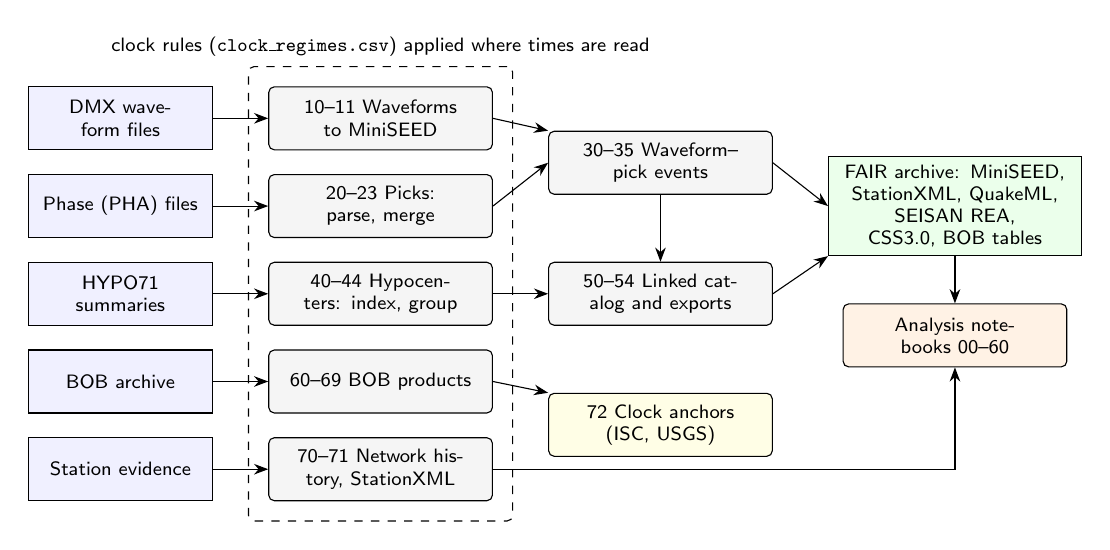
\begin{tikzpicture}[
  stepbox/.style={draw,rounded corners=2pt,align=center,font=\sffamily\scriptsize,minimum height=8mm,text width=27mm,inner sep=2pt,fill=gray!8},
  srcbox/.style={draw,align=center,font=\sffamily\scriptsize,minimum height=8mm,text width=22mm,inner sep=2pt,fill=blue!6},
  prodbox/.style={draw,align=center,font=\sffamily\scriptsize,text width=30mm,inner sep=3pt,fill=green!8},
  arr/.style={-{Stealth[length=1.8mm]},thin},
  node distance=3mm and 7mm]
\node[srcbox] (dmx) {DMX waveform files};
\node[srcbox,below=of dmx] (pha) {Phase (PHA) files};
\node[srcbox,below=of pha] (hyp) {HYPO71 summaries};
\node[srcbox,below=of hyp] (bob) {BOB archive};
\node[srcbox,below=of bob] (sta) {Station evidence};
\node[stepbox,right=of dmx] (s10) {10--11 Waveforms to MiniSEED};
\node[stepbox,right=of pha] (s20) {20--23 Picks: parse, merge};
\node[stepbox,right=of hyp] (s40) {40--44 Hypocenters: index, group};
\node[stepbox,right=of bob] (s60) {60--69 BOB products};
\node[stepbox,right=of sta] (s70) {70--71 Network history, StationXML};
\node[stepbox,right=of s20,yshift=5.5mm] (s30) {30--35 Waveform--pick events};
\node[stepbox,right=of s40] (s50) {50--54 Linked catalog and exports};
\node[stepbox,right=of s60,yshift=-5.5mm,fill=yellow!10] (s72) {72 Clock anchors (ISC, USGS)};
\node[prodbox,right=of s30,yshift=-5.5mm] (fair) {FAIR archive: MiniSEED, StationXML, QuakeML, SEISAN REA, CSS3.0, BOB tables};
\node[stepbox,below=6mm of fair,fill=orange!10] (an) {Analysis notebooks 00--60};
\node[draw,dashed,rounded corners=2pt,fit=(s10)(s70),inner sep=2.5mm,label={[font=\sffamily\scriptsize]above:{clock rules (\texttt{clock\_regimes.csv}) applied where times are read}}] {};
\draw[arr] (dmx)--(s10); \draw[arr] (pha)--(s20); \draw[arr] (hyp)--(s40); \draw[arr] (bob)--(s60); \draw[arr] (sta)--(s70);
\draw[arr] (s10.east)--(s30.north west); \draw[arr] (s20.east)--(s30.west);
\draw[arr] (s30)--(s50); \draw[arr] (s40)--(s50);
\draw[arr] (s50.east)--(fair.south west);
\draw[arr] (s60.east)--(s72.north west);
\draw[arr] (s30.east)--(fair.west);
\draw[arr] (s70.east)-|(an.south);
\draw[arr] (fair)--(an);
\end{tikzpicture}
\caption{Conversion workflow and its products. Sources (blue) are converted by numbered notebooks (gray); every step that reads raw times applies the clock rules (dashed box). Waveforms and picks are joined into events (30--35) and then linked with hypocenters (50--54). StationXML (70--71) is built last, once every stream is on UTC. Step 72 checks absolute time against global catalogs using the waveforms, picks, hypocenters and SSAM. The analysis notebooks (00--60) read the converted waveforms and station metadata.}
\label{fig:workflow}
\end{figure*}

\begin{table*}
\tbl{Conversion steps.\label{tab:steps}}
{\begin{tabular*}{\textwidth}{@{\extracolsep{\fill}}lp{0.73\textwidth}@{}}
\toprule
\textbf{Step} & \textbf{Purpose} \trowsep
10 & DMX to MiniSEED in a SEISAN WAV database; UTC start times; waveform index, per-file log, failures table; partial-file recovery \trowsep
11 & Daily file counts and station availability \trowsep
20--23 & Parse single-event and monthly phase files; merge them and suppress duplicates; pick and cross-source diagnostics \trowsep
30--35 & Match picks to the waveform records that contain them; build waveform and pick-only event containers; diagnostics \trowsep
40--44 & Index both HYPO71 summaries; compare them; group origins and choose a preferred origin; daily counts \trowsep
50--54 & Linked ObsPy catalog (QuakeML) with composition classes; reporting windows; SEISAN REA; Antelope CSS3.0 \trowsep
60--69 & Unpack the BOB archive; one notebook per product (RSAM/EVNT, SSAM, tilt, rain, mudflow, COSPEC, counts, radio maps); coverage overview \trowsep
70--71 & Network history, channel epochs on UTC and StationXML; validation \trowsep
72 & Absolute clock anchors from ISC and USGS events \\
\botrule
\end{tabular*}}
{}
\end{table*}

\subsection{Waveforms (steps 10--11)}

FloVoPy reads each DMX file, removes the IRIG trace, subtracts the 2,048-count digitizer offset, maps legacy component codes to SEED identifiers (for example \texttt{PPOZ} to \texttt{XB.PPO..EHZ}; the low-gain \texttt{PI2L} becomes \texttt{XB.PI2..ELZ}), converts the start time to UTC with the waveform rules, and writes MiniSEED into a SEISAN WAV database \citep{Havskov_1999}. The header sample rate, 100.80645~Hz, is kept as 3125/31~Hz rather than rounded to 100~Hz, which would have stretched every record by 0.8\%. Every one of the 21,475 DMX files is accounted for in a per-file log: 21,459 converted, 11 failed and 5 empty (two contain only flat or IRIG traces, three are header-only). Ten damaged files keep the complete traces before their first defect, and the index records the recovery. The 21,459 files hold 152,933 traces; dropped traces (16,586 flat, 514 IRIG, 25 with no samples) are kept as provenance rows rather than silently removed. By clock rule, 1,266 files precede the 26 May reset, 18,919 fall in U.S. daylight time and 1,274 after it. Figure~\ref{fig:stations} shows which stations are present in the converted records each day.

\begin{figure*}
\centering
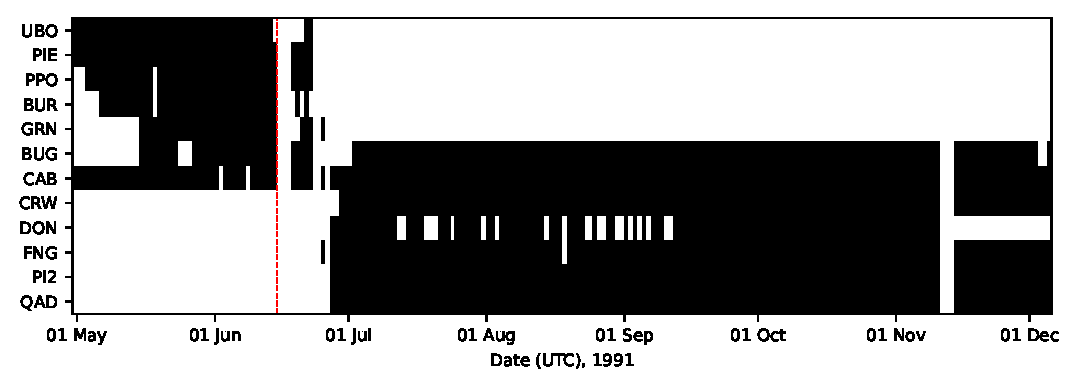
\includegraphics[width=\textwidth]{fig_station_availability}
\caption{Daily station presence in the converted triggered waveforms (black: at least one record), on UTC days. This is file availability, not continuous station operation. The dashed line marks 15 June.}
\label{fig:stations}
\end{figure*}

\subsection{Phase picks (steps 20--23)}

All phase-card decoding is in FloVoPy, with tests on historical excerpts. Fixed-column decoding repaired several silent errors in earlier parsers: S-only cards whose minute was read from the wrong columns; minute-60 and seconds-$\ge$60 cards, which HYPO71 allows and which are now rolled over (114 lines); and S readings with seconds just below the P seconds, which an earlier rule moved one minute later. None of the 34 such cards is a genuine minute wrap: analysts wrote later S times as seconds $\ge$ 60 (506 cards), so an S earlier than its P is now logged and skipped. Monthly blocks missing a separator line are split where picks are more than 20~s apart and each piece has at least three stations (12 blocks). The single-event files give 1,328 picks in 119 events and the monthly files 57,333 picks in 8,230 events; merging suppresses 593 duplicates and leaves 58,068 picks.

\subsection{Waveform--pick events (steps 30--35)}

Each single-event pick group is matched to the one waveform record that encloses it, and each monthly block is attached as a whole to the record containing most of its picks. Picks that duplicate another source within an event (1,413, mostly repeated copies of the same event in the monthly files) are suppressed and recorded, so they cannot resurface as pick-only events. The result is 21,691 containers: 7,715 with waveform and picks, 13,744 waveform-only and 232 pick-only. Every pick appears exactly once, either in a container or in the suppressed table.

\subsection{Hypocenters (steps 40--44)}

The two summaries are parsed separately with a FloVoPy HYPO71 reader, converted to UTC, and kept with source and line provenance (8,233 origins). A magnitude of 0.00 means none was computed (1,806 summary rows and 960 \file{PINAALL.DAT} rows) and is stored as missing with the reported value retained. Origins are grouped into 4,690 events; a stable sort keeps equal times in input order. Each group has a preferred origin chosen by a stated source policy, which is a curation choice, not evidence that one solution is more accurate; it changes the preferred origin in 608 of 3,507 two-source groups. Figure~\ref{fig:hypo} shows the preferred solutions. They are not relocated.

\begin{figure*}
\centering
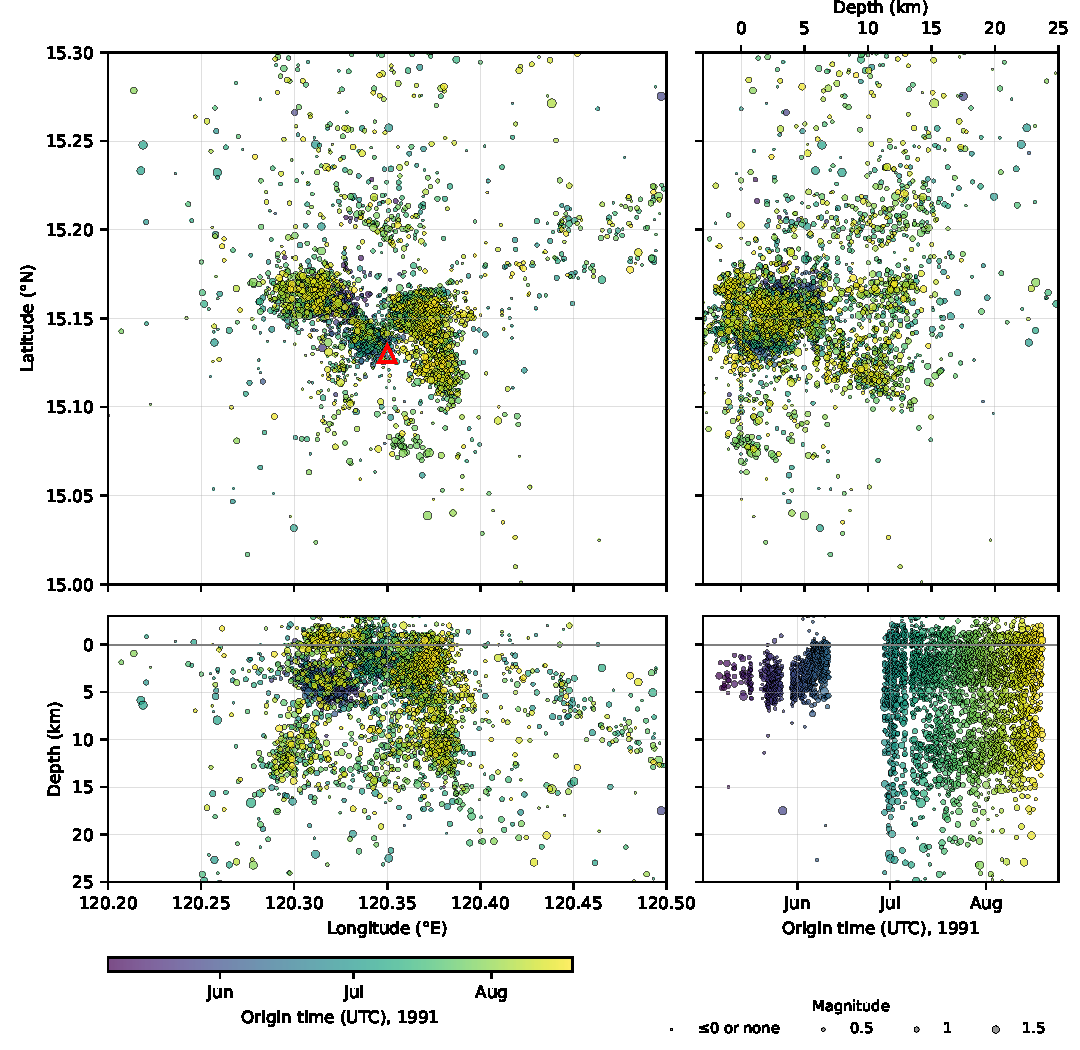
\includegraphics[width=\textwidth]{fig_hypocentres}
\caption{Preferred solutions of the 4,690 hypocenter groups: map view (top left) with latitude--depth (top right), longitude--depth (bottom left) and depth--time (bottom right) sections, colored by origin time (UTC). Symbol area scales with magnitude; magnitudes of 0.0 and below, and missing magnitudes (1,306 groups), are drawn at the smallest size. Catalog depths are shown as reported, including negative values; no relocation or quality filtering is applied. 131 solutions fall outside the map and 14 are deeper than 25~km. Gray contours (200~m interval) and the brown profiles (east--west and north--south through the summit, elevation plotted as negative depth) are modern relief, which postdates the 1991 eruption and lies about 250~m below the pre-eruption summit. The triangle marks the summit.}
\label{fig:hypo}
\end{figure*}

\subsection{The linked catalog (steps 50--54)}

Step 50 builds one ObsPy catalog. Hypocenters are linked to events first through their picks: a hypocenter links to the event whose first P arrives 0--10~s after the origin, closest to the expected 1.7~s. Remaining hypocenters link to the waveform record whose window, extended 10~s before its start, contains the origin. Both stages are one-to-one. An earlier rule that required the origin within $\pm$10~s of the record start failed for about 40\% of pairs, because records start about 11~s before the first arrival and origins fall a median 9.5~s after the start. The new rule links 4,628 of the 4,690 hypocenters (4,446 through picks, 182 by window); 46 of the remaining 62 lie inside a record already linked to another hypocenter, typically two earthquakes in one file.

Each event records which of waveform (W), picks (P) and hypocenter (H) survive (Table~\ref{tab:classes}). The catalog has 21,753 events, 8,233 origins, 56,655 arrivals and magnitudes for 3,414 events. QuakeML \citep{Schorlemmer_2011} carries origin time errors from the clock rules and a comment with the rule and raw time. A SEISAN REA database holds one S-file per event; FloVoPy repairs three faults in ObsPy's Nordic writer (origin seconds written as the first digit of the microseconds, a missing magnitude type written as ``W'', and an RMS always written as zero) and keeps a manifest so that reruns reuse unchanged files and never overwrite untracked ones. An Antelope CSS3.0 export holds origins, arrivals, associations and network magnitudes. Step 51 derives reporting windows in which all three sources are present, 8 May--10 June and 29 June--18 August, containing 11,753 events, and gives daily counts by class (Fig.~\ref{fig:daily}).

\begin{table}
\tbl{Composition of the 21,753 catalog events by surviving source.\label{tab:classes}}
{\begin{tabular*}{\columnwidth}{@{\extracolsep{\fill}}lr@{}}
\toprule
\textbf{Class} & \textbf{Events} \trowsep
Waveform, picks and hypocenter (W+P+H) & 4,353 \trowsep
Waveform and picks (W+P) & 3,362 \trowsep
Waveform and hypocenter (W+H) & 154 \trowsep
Waveform only (W) & 13,590 \trowsep
Picks and hypocenter (P+H) & 121 \trowsep
Picks only (P) & 111 \trowsep
Hypocenter only (H) & 62 \\
\botrule
\end{tabular*}}
{}
\end{table}

\begin{figure*}
\centering
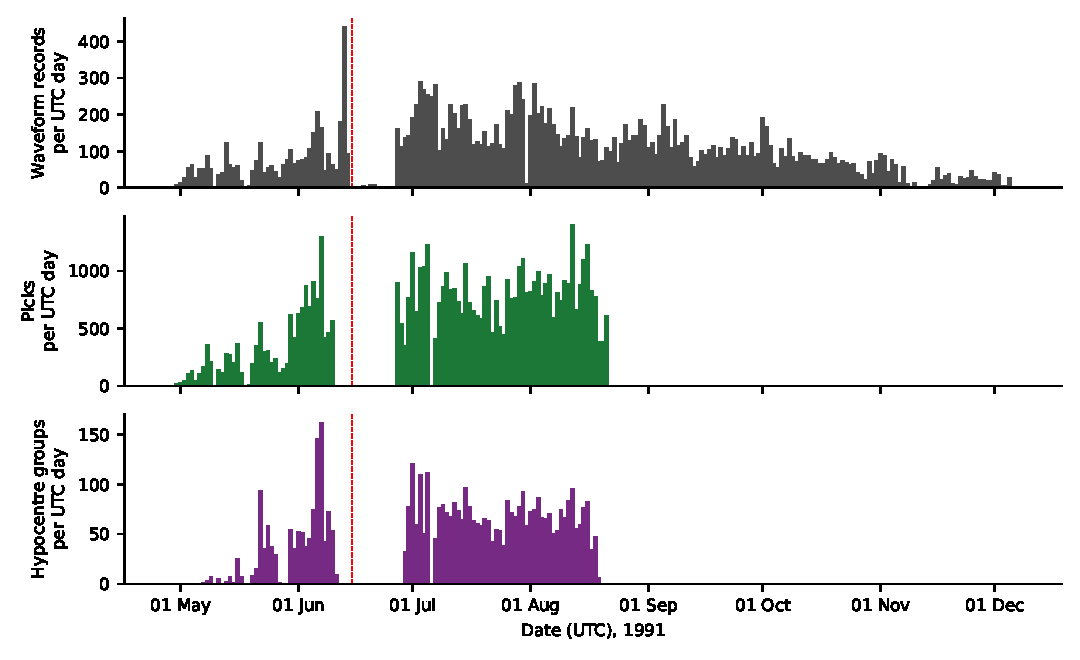
\includegraphics[width=\textwidth]{fig_daily_counts}
\caption{Daily counts on UTC days of converted waveform records (21,459), merged picks (58,068) and hypocenter groups (4,690). These are different counting units, not counts of distinct earthquakes. The dashed line marks 15 June.}
\label{fig:daily}
\end{figure*}

\subsection{BOB products (steps 60--69)}

Step 60 unpacks the BOB archives (by default only previewing; it is the only step that changes the legacy inputs). Steps 61--68 convert one product each, with FloVoPy readers, the product's clock rule and a common set of quality outputs (coverage, daily coverage, date review, review flags and export status). Product-specific checks include: RSAM, EVNT and tilt windows labeled at their end; all-zero SSAM rows treated as dropouts (36,037 of 635,862 rows); rain values repeated from the previous row flagged as carried forward, because the historical converter rewrote every channel's last value; the tilt digitizer limit (8,192) masked; and auxiliary test channels excluded from coverage. Step 69 summarizes network-wide coverage (Fig.~\ref{fig:bob}) and compares RSAM with summed SSAM day by day (Fig.~\ref{fig:drift}).

\subsection{Station metadata (steps 70--71)}

Step 70 reconstructs the network history from field notes, maps and the converted archive, and writes StationXML. It runs last, after every stream is on UTC. Field-note dates are Philippine local time and are converted: a date-only bound becomes local midnight (16:00 UTC the previous day). Where the archive contradicts the documents, the archive decides the epoch, and the difference is recorded: UBO data precede its documented installation, and several stations keep their labels for 6--10 days after their documented ends, so those traces get their own epoch with an unknown sensor. The result has 13 stations and 33 channel epochs at 3125/31~Hz, schema-valid, and every one of the 152,933 archived traces falls inside an epoch of its identifier; the build fails otherwise. Responses are nominal models of the sensors and attenuation settings, marked as having unknown electronics; they are not end-to-end calibrations. Step 71 checks the saved products and runs controlled reconstruction tests.

\subsection{Testing and provenance}

The conversion has 77 tests: clock rules, phase-card parsing and comparison, the catalog, REA and CSS3.0 export semantics, the BOB products and the network reconstruction, loading notebook functions from their definition cells. FloVoPy has its own suite of more than 200 tests. Each product records its inputs, configuration and code; for example, the StationXML provenance records the hashes of the notebook, the configuration and the waveform index.

\section{Analysis Workflow}

A second notebook sequence (\file{20\_analysis}, notebooks 00--60) measures noise and event windows across the converted archive. It reads the UTC waveforms and copies the step-70 station metadata with their hashes; it never rebuilds them.
\begin{itemize}
\item \textbf{00, inventory and quality control.} For every trace: original-sample coverage, length, padding, gaps, extrema, repeated values and a narrowband screen at 40.5~Hz, an acquisition artifact.
\item \textbf{10, station metadata.} A read-only copy of the step-70 products, matched to each trace's channel epoch.
\item \textbf{20, window selection.} The default fixed policy takes the first 5~s of each trace as noise and the rest of the record as event data. A detected policy instead uses FloVoPy's pretrigger detector: a network-wide onset supported by at least two stations, a trace-specific onset, and a noise prefix ending 1~s before it, shortened by any earlier activity. A reviewed policy uses analyst decisions. This notebook also shows the onset histogram and frequency and instantaneous-frequency diagnostics for example records.
\item \textbf{30, metrics.} For each noise and event window: amplitude statistics, band-limited mean absolute amplitude and energy (0.8--4 and 4--20~Hz), temporal, shape, spectral and cepstral features from FloVoPy, and matched Welch \citep{Welch_1967} and equal-weight multitaper \citep{Thomson_1982} power spectral densities on the same segments. Values are in uncalibrated counts.
\item \textbf{40--60.} Spectra and spectrograms at several resolutions, archive summary figures, and publication figures from an explicitly selected set of examples.
\end{itemize}
Full results are stored per recording as JSON sidecars holding every array, window choice, feature, quality flag and provenance, under a computation signature, so unchanged recordings are reused when selections or plots change. A fixed-schema table supports plotting, and a full export flattens every field into a compressed Parquet file. Each run has an identifier derived from the configuration, the selected files and the hashes of the workflow and FloVoPy code. The current full-archive run reads all 21,459 files and 152,933 traces on 15 channel identities and measures 305,866 windows. These windows are conditioned on triggering: the noise reference precedes a detected event and is not an unbiased survey of ambient noise, and an event window ending at the record boundary is not a measured coda duration.

\section{Example: Frequency Content before the 15 June Eruption}

Putting every stream on UTC lets products from different acquisition computers be read together. Figure~\ref{fig:june} shows 1--15 June 1991 on one UTC time axis. The waveform panels use the event windows of the full-archive analysis run (fixed policy) at PIEZ and GRNZ, the two vertical channels that recorded continuously until 14 June. Windows flagged for possible clipping (15) or with an event-to-noise amplitude ratio below 6~dB are excluded, leaving 2,784 of 3,658 windows (1,467 at PIE, 1,317 at GRN). The frequency index is the base-2 logarithm of the ratio of mean absolute amplitudes in the 4--20 and 0.8--4~Hz bands \citep[after][]{Buurman_2010}, and the spectral centroid is the power-weighted mean frequency of the Welch spectrum.

Both measures fall through early June at both stations. At PIE the median frequency index drops from 0.43 for 1--5 June to $-$0.66 for 9--14 June and the median centroid from 8.6 to 4.0~Hz, mostly in steps on 7 and 8--9 June; at GRN the index drops from 0.94 to 0.02 and the centroid from 6.3 to 4.7~Hz. The shift toward lower frequencies matches the hybrid and long-period events that appeared from 8 June in the analog records \citep{Harlow_1996} and the growth of 0.5--2.5~Hz energy that \citet{Power_1996} describe in SSAM. The HYPO71 magnitudes (517 of the 752 hypocenter groups in this interval have one) show no comparable trend, and no events were located between 11 June and the climactic eruption. RSAM at PIEZ, recorded by the Tandy computer on its own clock, rises abruptly in the 10-minute sample that contains 00:51~UTC on 12 June, the time of the first large explosive eruption \citep{Wolfe_1996}, and stays high until the station was lost on 15 June; this agreement is an independent check of the RSAM clock rules. SSAM, from WILLIE, survives for June only on 11 June (BUR) and from 12 June (CAB); its amplitude is concentrated in the lowest bands and grows toward 15 June.

This example is descriptive. The station set, triggering and window policy all shape the values, amplitudes are uncalibrated counts, and a physical interpretation of the frequency change is left to later work; like every figure here, it is produced from the archived products by a notebook in the repository.

\begin{figure*}
\centering
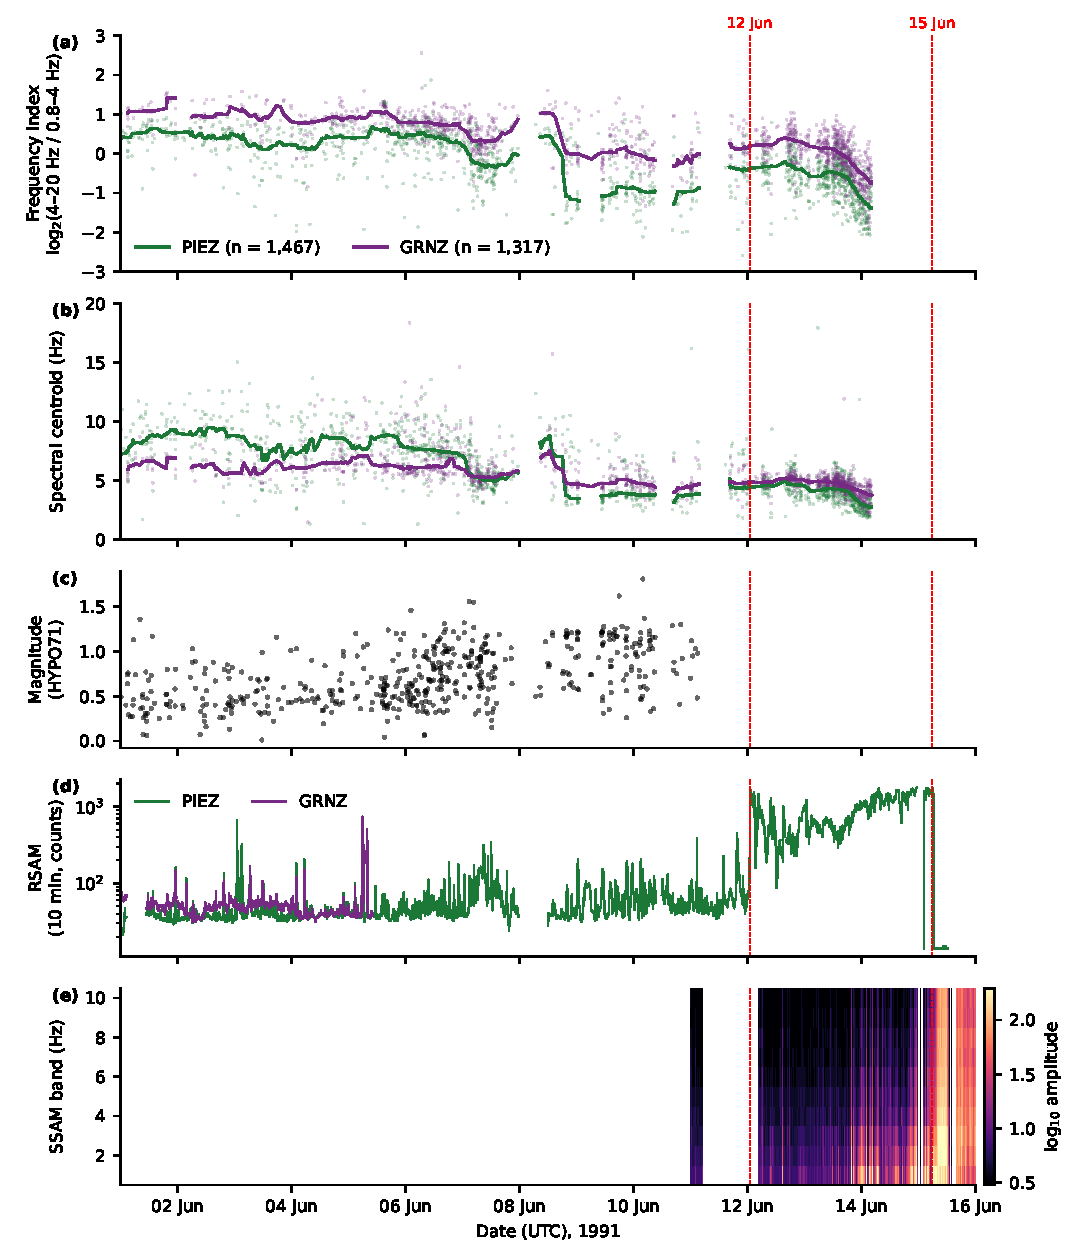
\includegraphics[width=\textwidth]{fig_june_frequency}
\caption{1--15 June 1991 on one UTC time axis. (a) Frequency index, $\log_2$ of the 4--20~Hz to 0.8--4~Hz mean-absolute-amplitude ratio, and (b) spectral centroid of each retained event window at PIEZ (green) and GRNZ (purple), with 12-hour running medians (broken across gaps of more than 6~h). (c) HYPO71 preferred magnitudes. (d) RSAM, 10-minute averages, at PIEZ and GRNZ. (e) SSAM bands BN01--BN10 (0.5--10.5~Hz), BUR on 11 June and CAB from 12 June. Dashed lines mark the first large explosive eruption (00:51~UTC, 12 June) and the climactic eruption (about 05:42~UTC, 15 June) \citep{Wolfe_1996}.}
\label{fig:june}
\end{figure*}

\section{Limitations and Reuse}

The archive supports reassessment of captured events, of historical processing, and of the relationships among monitoring products. Several limits remain.
\begin{itemize}
\item \textbf{Sampling.} Triggered recording does not sample all seismicity. A missing family during a swarm may reflect triggering or preservation, and waveform-file counts are not earthquake counts.
\item \textbf{Absolute time.} Hour-scale offsets are corrected, but drift is not. Absolute times carry an uncertainty of about 25~s after 26 May and 60~s before; relative timing within a file is unaffected. Rain and mudflow after 15 November and RSAM from 2 to 9 May rest on weak or no evidence.
\item \textbf{Calibration.} Responses are nominal; amplitudes are in counts. Comparisons across stations, gain epochs or attenuation changes need care.
\item \textbf{Locations.} The hypocenters are historical solutions, not relocated, and the choice of preferred origin is a curation policy.
\item \textbf{Helicorders.} The drum records are images with a separate clock and are not digitized.
\end{itemize}
A constant absolute-time offset does not change waveform shape or spectral content within a window, so waveform-based studies are largely unaffected by the residual clock error; comparisons with external catalogs or other observatories need the stated uncertainty.

\section{Conclusions}

Most of the difficulty in recovering the 1991 Pinatubo record lay not in file formats but in time. Each acquisition computer kept its own clock, the clocks used Philippine time or GMT at different times, and the seismic acquisition software applied a California time-zone conversion. Reconstructing that history from file order, header fields and cross-correlation, and encoding it as explicit, documented rules, brings the streams into agreement: 97.3\% of hypocenters now fall inside a waveform record, against 12.9\% before. Regional and teleseismic arrivals bound the residual absolute error to tens of seconds, and a worked example shows waveform frequency content, magnitudes, RSAM and SSAM from separate computers read together through the June 1991 crisis. The linked catalog records for each of 21,753 events which observations survive, and the station metadata, monitoring products and catalog exports are built by open, tested workflows that keep the raw values and the evidence beside every correction. The same approach, which treats each acquisition clock as a separate stream with documented rules, should transfer to other early-digital volcano networks.

\begin{datres}
The assembled data are EarthScope Assembled Dataset 25-028 (PIN 1991 FAIR), associated with temporary network XB (1991), network DOI 10.7914/seq1-hh72 \citep{XB_1991}. The scanned drum records are USGS data release 10.5066/P13DUU3H \citep{Power_2025}. The conversion and analysis notebooks are at \url{https://github.com/gthompson/Pinatubo1991SeismicData} and the FloVoPy library at \url{https://github.com/gthompson/flovopy} (last accessed November 2026; the revisions used will be archived with a DOI at publication). All figures in this paper are made by the notebook \file{papers/SRL/make\_figures.ipynb} from the conversion and analysis products. The supplemental material for this article describes the monitoring system and the telemetry, gives the HYPO71 control file and velocity model, the complete clock rules, further clock evidence, coverage of every channel and product, and checks on the picks, locations and catalog; its figures are made by \file{papers/SRL/supplement/make\_supplement.ipynb}. Global earthquake catalogs were obtained from the ISC \citep{ISC_2024} and USGS \citep{USGS_2017} FDSN event services through ObsPy \citep{Beyreuther_2010,Krischer_2015}; travel times use TauP \citep{Crotwell_1999} and iasp91 \citep{Kennett_1991}. The updated products described here (UTC waveforms, catalog exports, StationXML and BOB tables) are not yet in the assembled release; they will be deposited as a new version of the XB (1991) dataset \citep{XB_1991}.
\end{datres}

\section{Declaration of Competing Interests}

The authors acknowledge that there are no conflicts of interest recorded.

\begin{ack}
We thank the PHIVOLCS and VDAP personnel who installed, operated and interpreted the monitoring systems during the crisis and those who preserved the records afterward. Thomas Murray recovered the BOB archive and explained its acquisition system. OpenAI Codex and Anthropic Claude assisted with source inspection, code, product accounting, figure preparation and drafting; the authors are responsible for verifying the manuscript, calculations and figures.
\end{ack}

\bibliography{pinatubo}

\end{document}
